\section{Module Functions and Integration}
\label{sec:modules}
The architecture in Fig.~\ref{fig:arch} is implemented as cooperating
modules rather than a single monolithic agent. Shared interfaces connect
task execution to configuration, industrial services, protocol drivers, and
route-specific evidence. This section describes those responsibilities and
the checks that preserve their boundaries.

The extension contracts expose the data passed at each boundary. A harness
call is normalized as \texttt{HostToolCall(toolName, arguments)} and returns
\texttt{HostToolResult(text, isError)}. A DCW driver accepts an engineering
value, tolerance, range, and driver configuration; its result separates write
status, raw value, readback, and acknowledgment grade (readback-verified,
transport-ack, or unverified). Each DAQ sample stores its node, timestamp,
value, and state, with optional line, product, recipe, and run IDs. A write
anchor records line/node, prior and requested values, source, actor, time, and
optional run/task/approval IDs; recipe definitions retain separate versions.
These fields keep tool errors, device receipts, observations, and production
lineage inspectable as separate records.

\subsection{Task Runtime and Harness Adapters}
An access surface creates or joins a workspace channel, where the task
engine manages members, task queues, shared memory, and execution templates.
The harness registry instantiates an adapter behind a common agent interface;
the prompt builder combines the task with the active scene brief, industrial
context, channel profile, agent binding, and retrieved memory. Tool calls
return to the shared dispatcher regardless of which registered harness
produced them. The registry is an extension point; the experiments do not
establish portability across harnesses.

\subsection{Production Context and Configuration}
Scene blueprints describe devices, signal maps, objectives, and process
guards. A task resolves these definitions against its active
line--product--recipe--run context. The channel profile selects the available
capability family, the tool policy narrows the operation catalog, and the
agent binding scopes the nodes, controls, and recipe operations available to
that member. These filters can restrict one another but cannot broaden the
underlying device range. The dispatcher re-reads policy at execution, so a
cached catalog does not retain authority after a grant or policy change.

\subsection{Acquisition, Analysis, and Modeling Services}
Semantic DAQ nodes expose typed values, engineering units, ranges, and
sampling settings while hiding protocol-specific reads. A per-node DAQ
runtime schedules acquisition and stores timestamped observations; the
gateway aggregates node pipelines. MES-facing operations provide the
configured production-data path. Analysis and retrieval services consume
these records, while optional model, training, optimization, and digital-twin
services are invoked through their registered operation handlers. These
services complement the agent workflow; AgentWorkShop does not prescribe a
single optimization strategy.

\subsection{Semantic I/O and Actuation}
The driver registry resolves a semantic node to a built-in or plugin driver.
DAQ handlers use the node's acquisition interface; DCW handlers route a
write or readback through the controller and the configured protocol driver.
This separation lets recipes and agents refer to semantic controls without
embedding Modbus, OPC UA, MQTT, HTTP, or MES transport details in their
operation arguments. The supported driver mappings are implementation
interfaces; only the mappings and workflows enumerated in Section~\ref{sec:eval}
are experimentally exercised.

\subsection{Shared Dispatch and Write Admission}
\label{sec:governed}
Every named operation passes the dispatcher. Its ordered checks validate
invocation scope, channel tool selection, profile, duty separation, the
agent's binding and runtime grant, and ownership of referenced resources.
A refusal returns the excluding condition and is recorded. A catalog entry
therefore describes availability but does not authorize execution. Handlers
for operations that require manual approval suspend for a decision, then
revalidate authority and active limits before dispatch.

All actuator writes converge on the DCW admission point. For an online node
write, the admissible interval is
\begin{equation}
\mathcal{I}^{\mathrm{online}}_n(t)=\mathcal{H}_n\cap\mathcal{B}_n
\cap\mathcal{P}_n(t)\cap\mathcal{R}_n(t),
\label{eq:admission}
\end{equation}
where $\mathcal{H}_n$ is the hard engineering range and $\mathcal{B}_n$,
$\mathcal{P}_n$, and $\mathcal{R}_n$ are the baseline, active-product, and
active-recipe limits. Missing optional limits impose no restriction, whereas
an empty intersection rejects the request and identifies the excluding
layer. Recipe dispatch applies the hard, baseline, and product limits to the
replacement recipe rather than intersecting with the previous recipe window.
The actuator path also enforces step, interval, and hold-window checks.
These admission rules constrain commands; process objectives and coupled
variable guards are assessed from later observations. The framework does
not replace independent PLC or safety-instrumented protection.

\subsection{Integrated Operation and Route-Specific Evidence}
\label{sec:tasklifecycle}
A recipe trial illustrates how the modules cooperate. The task runtime
delivers a named \texttt{recipe\_trial} call from the agent harness; the
dispatcher checks the agent's recipe binding and execution scope; the recipe
handler checks the active run, candidate parameters, and route timing; and a
manual binding requests approval before the DCW controller sends the batch
through its driver. The handler returns a per-parameter receipt. The caller
then obtains DAQ observations and can request a separate update, apply, or
rollback operation. A trial receipt confirms command handling; it does not
by itself establish process attainment or persist a new recipe version.

The routes retain different records because they answer different
questions. A driver acknowledgment reports command evidence; DAQ reports a
process observation; an exploration summary records a bounded probe; and a
recipe version records a saved definition. Their relation through actor and
production context allows an execution to be inspected without treating
these outcomes as interchangeable.

\subsection{Route-Specific Lifecycles and Evidence}
\label{sec:routes}
\label{sec:mech}
\label{sec:objective}
\label{sec:nodeexec}
\label{sec:ack}

\paragraph{Timing and approval}
Timing guards are route-specific. Online node writes enforce an effective
minimum spacing of 60\,s. Recipe dispatch uses a per-recipe interval anchored
to approval, while trials also use a configurable per-line cadence (default
300\,s). The recipe interval can refuse a proposal before an approval request
is created. Checks occur at proposal or execution according to the operation,
and experiment-specific pacing overrides are reported with the corresponding
results.

Manual bindings create an approval request containing the actor, node or
recipe, candidate values, applicable limits, expiry, and parameter bases.
The default wait expires after 180\,s and refuses execution. After approval,
the executor rechecks authorization and active limits to account for context
changes during the wait. For \texttt{recipe\_apply}, a changed definition
requires a new proposal; an unchanged approval dispatches a copy of the
approved parameter snapshot. A line-level recipe mode defaults to manual;
changing it to automatic requires administrator confirmation. The approval
record authorizes a workflow action and does not replace process protection.

\begin{figure*}[!t]
\centering
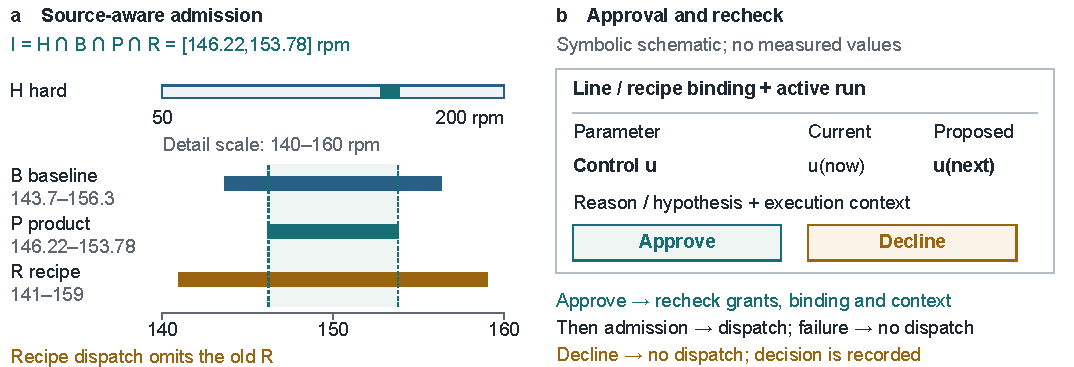
\includegraphics[width=\textwidth]{resources/fig-admission-hitl-2026.pdf}
\caption{Admission and approval boundaries. (a) Archived Q1 RPM example:
online node interventions use the four-layer value interval of Eq.~(1),
whereas recipe dispatch omits the prior recipe window. (b) Symbolic human
approval binds a proposed action and authority fields; execution checks run
again after approval, which does not reserve equipment state.}
\label{fig:hitl}
\end{figure*}

\paragraph{Node probe}
The bounded node probe is exposed as \texttt{optimization\_explore} to the
Auto Modeling Lab (AML) optimization profile (\texttt{aml\_optimization}).
The profile validates a bound control and target DAQ scope,
captures a starting control and target baseline, invokes the internal DCW
write path, then waits 10--300\,s (default 45\,s) and queries a trailing 45-s
target window before saving an exploration summary. Since each window is
relative to its query time, approval can separate baseline sampling from
actuation; a 10-s wait can leave about 35\,s of pre-write samples in the later
window. The command receipt and target summary are therefore returned
separately. A successful changed-value write opens a node-optimization
record; refusal or expired approval creates a rejected summary without a
post-write sample.

\paragraph{Recipe operations}
\texttt{recipe\_trial} checks the bound recipe and active run, then dispatches
candidate overrides as a batch with per-parameter verification. The caller
subsequently queries DAQ and decides whether to save a new definition with
\texttt{recipe\_update}, restore one with \texttt{recipe\_rollback}, or
dispatch a version with \texttt{recipe\_apply}. These steps are separate: a
trial does not save or apply a version, and endpoint verification is not a
process-response measurement. Public direct-node control is closed; the
bounded probe and recipe operations are the configured operation surfaces.
The historical four-scene results use an earlier direct-node path and do not
test current profile or binding adaptation across scenes.

\paragraph{Command verification}
Command confirmation and process response answer different questions. A
driver ACK is graded as \texttt{readback-verified}, \texttt{transport-ack},
or \texttt{unverified}. A matching endpoint read supports the first grade; a
transport or MES application receipt supports the second. Recipe batch
verification assigns \texttt{verified}, \texttt{unverified}, or
\texttt{failed}; if no matching readback is available, it attempts up to
three independent reads, 2\,s apart. A matching retry upgrades the final ACK,
while exhausted retries remain unverified. The initial ACK remains in write
history and the final ACK and verdict are retained with the batch.
Per-parameter receipts preserve successful outcomes when another parameter
fails. A readback-verified setpoint does not establish target attainment.

\paragraph{Observation, verdict, and compensation}
The caller performs recipe-path observation after batch dispatch. The October
recipe case therefore compares a recipe definition, endpoint readback, and
DAQ sample as separate representations. Saving a definition, applying it to
equipment, and observing its process response are separately evidenced
operations. The evaluation does not combine these route-specific records into
one universal end-to-end record.

An open node record provides a monitoring backstop. After 120\,s it polls
every 30\,s; three cumulative samples outside the recipe monitoring window
trigger a system-attributed rollback request toward the preceding value.
Missing samples do not count as breaches. A caller's \texttt{keep},
\texttt{rollback}, or \texttt{uncertain} verdict records its interpretation;
compensation is a new command subject to its applicable admission policy.
The write audit deduplicates the same value on the same node within 10\,s,
while batch receipts, exploration summaries, DAQ history, and recipe versions
retain their distinct lifecycles. Linking these records by actor and
production context allows the command, endpoint evidence, and process
observation to be inspected without treating them as interchangeable.
\label{sec:agentloop}

